\documentclass[addpoints,12pt,answers]{exam}
\usepackage{babel}
\usepackage[top=3cm,bottom=3cm,left=2.5cm,right=2.5cm]{geometry}
\usepackage[utf8]{inputenc}
\usepackage[T1]{fontenc}
\usepackage{booktabs}
\usepackage{graphicx}
\usepackage{csquotes}
\usepackage{paralist}
\usepackage{wasysym}
\usepackage[math]{iwona}
\usepackage{setspace}
\usepackage{enumitem}
\usepackage{multirow}
%\usepackage{mathtools}
%\usepackage{array, amssymb}

\pointpoints{Point}{Points}
\bonuspointpoints{Bonuspunkt}{Bonuspunkte}
\renewcommand{\solutiontitle}{\noindent\textbf{Solution:}\enspace}

\chqword{Frage}   
\chpgword{Seite} 
\chpword{Punkte}   
\chbpword{Bonus Points} 
\chsword{Erreicht}   
\chtword{Gesamt}

\checkboxchar{\Square}
\checkedchar{\CheckedBox}

\pagestyle{headandfoot}
%\runningheadrule
%\firstpageheader{ECO208}{Test 3}{28th Feb, 2022}
%\runningheader{ECO208}{Test 3}{28th Feb, 2022}
%\firstpagefooter{ECO208}{Test 3}{\thepage\,/\,\numpages}
%\runningfooter{ECO208}{Test 3}{\thepage\,/\,\numpages}
\doublespacing

\begin{document}
	\vspace*{3em}
	
	\makebox[\textwidth]{ECO 209  Assignment 4 (tentative solution)}
	\makebox[\textwidth]{Name:\enspace\hrulefill}
	
	\vspace*{3em}
	
	\begin{questions}
				\question  [10]  The figure below shows two output gaps calculated from potential real gross domestic product, which were estimated by the Congressional Budget Office (CBO) in 2007 and 2018.  
		
		
		\begin{figure}[htbp!]
			\centering
			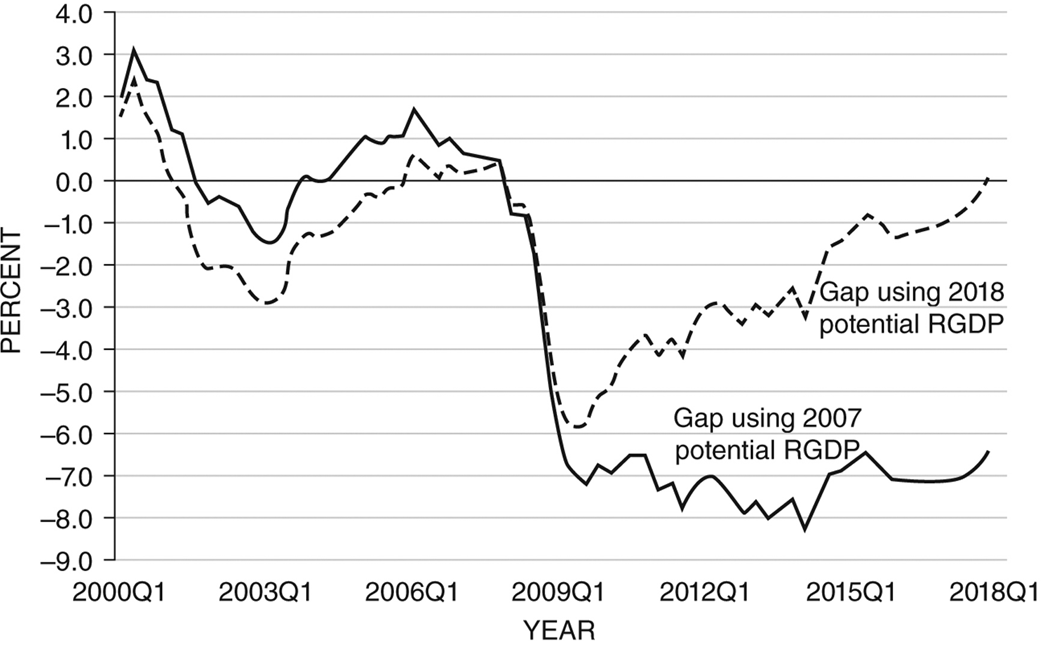
\includegraphics[width=0.6\linewidth]{figure/q3a}
		\end{figure}
		
		\begin{parts}
			\part [3] What explains the difference between the two gaps? Discuss in 2-5 sentences.
			\part [7] Suppose you are the chair of the Fed, how would that impact your choice of monetary policy if you think the right estimate is the 2007 version? How would it affect the monetary policy if you have the correct forecast ahead (the 2018 version)?
		\end{parts}
		\clearpage
		\begin{solution}
			\begin{parts}
				\part The CBO estimates of potential RGDP are adjusting to changes in actual data. Consequently, a slowdown in the economy results in a corresponding slowdown in potential real GDP (PRGDP). As the 2007 PRGDP does not yet account for the Great Recession, it would be higher than the PRGDP post-recession. The reduction in RGDP during the Great Recession contributes to a lower estimate of potential GDP in the subsequent years.
				
				\part  Continuing to rely on the 2007 estimates of potential GDP would result in a  larger output gap compared to using more recent data. As a result, the Fed may adopt overly aggressive measures to combat the recession, by lowering the interest rate. But, this could result in positive short-run output, potentially resulting in higher future inflation rates as the economy recovered. If the Fed has the more recent estimates, the Fed would first lower the interest rate then increase the interest rate gradually to counter any potential rise in inflation.
			\end{parts}
		\end{solution}
		
		\clearpage
		
	
		
		
		\clearpage
		\question  [20]  The economy can be described by the following equations:
		\begin{itemize}
			\item IS Curve: 
			\[
			\tilde{Y}_t = \bar{a} - \bar{b}(R_t-\bar{r})
			\]
			\item Phillips Curve: 
			\[
			\pi_{t} = \pi_{t-t} + \bar{\nu}\tilde{Y}_t + \bar{o}
			\]
			\item The central follows this Simple Monetary Rule:
			\[
			R_t - \bar{r} = \bar{m} \left(\pi_t - \bar{\pi}\right)
			\]
		\end{itemize}	
			
		Suppose the economy face a price shock of size \(\bar{o} >0\).
		
		\begin{enumerate}[label=(\alph*)]
			\item (3 pts) Derive the AD curve and AS curve.
			\item (4 pts) In the AS/AD graphs describing the economy's response to the inflation shock, we label the initial response of inflation as \(\pi_1\) and the initial output as \(\tilde{Y}_1\). What are the values of these key points in terms of the model parameters? In other words, by how much does output decline, and what is the initial inflation rate?
			
			\item (6 pts)Now suppose the AS and AD curves have the following parameter values:
			\[
			\bar{o} = 2\%, \quad
			\bar{a} = 0.5, \quad
			\bar{b} = \frac{1}{2}, \quad
			\bar{\nu} = \frac{1}{2}, \quad
			\bar{m} = \frac{1}{3}, \quad
			\bar{\pi} = 2\%.
			\]
			Solve for the value of short-run output and the inflation rate for the first three years following the shock.
			
			\item (7 pts) Draw a time path based on the value you calculated for $\tilde{Y}_t$, $R_t$ and $\pi$ (up to only first three periods). 
		\end{enumerate}
%		
		\clearpage
		\textbf{Solution}
		\begin{enumerate}[label=(\alph*)]
			\item (3 pts) 
			Plug in the Simple Monetary Rule into the IS curve:
			\[
			\tilde{Y}_t = \bar{a} - \bar{b}\bar{m} \left(\pi_t - \bar{\pi}\right)
			\]
			
			The AS curve is the Phillips Curve: 
			\[
			\pi_{t} = \pi_{t-1} + \bar{\nu}\tilde{Y}_t + \bar{o}
			\]
			
			\item (4 pts) In the AS/AD graphs describing the economy's response to the inflation shock, we label the initial response of inflation as \(\pi_1\) and the initial output as \(\tilde{Y}_1\). 
			
			\begin{figure}[hbtp!]
				\centering
				\includegraphics[width=0.5\linewidth]{"figure/q2 soln1"}
			\end{figure}
			
			We found the equilibrium by pluging in the AD curve into the AS curve (in particular, we sub in the $\tilde{Y}$):
			\[
			\pi_{t} = \pi_{t-1} + \bar{\nu}\left[\bar{a} - \bar{b}\bar{m} \left(\pi_t - \bar{\pi}\right)\right] + \bar{o}
			\]
			\clearpage
			Rearranging it:
			\[\pi_t = \left(\frac{1}{1+\bar{\nu}\bar{b}\bar{m}}\right) \left(\pi_{t-1}+\bar{\nu}\bar{a} + \bar{\nu}\bar{b}\bar{m}\bar{\pi} + \bar{o}\right)\]
			
			The AD curve becomes:
			\[\tilde{Y}_t = \bar{a} -\bar{b}\bar{m}\left(\left(\frac{1}{1+\bar{\nu}\bar{b}\bar{m}}\right) \left(\pi_{t-1}+\bar{\nu}\bar{a} + \bar{\nu}\bar{b}\bar{m}\bar{\pi} + \bar{o}\right)-\bar{\pi}\right)\]
			
			Update the time subscript and let $\pi_0=\bar{\pi}$ and $\bar{a}=0$:
			\[
			\pi_{1} = \bar{\pi} + \frac{\bar{o}}{1+\bar{\nu}\bar{b}\bar{m}} 
			\]
						
			Now, sub it into the AD curve:
			\[
			\tilde{Y}_1 = \bar{a} - \bar{b}\bar{m} \left(\pi_1 - \bar{\pi}\right) = - \bar{b}\bar{m} \left(\bar{\pi} + \frac{\bar{o}}{1+\bar{\nu}\bar{b}\bar{m}}  - \bar{\pi}\right) = - \frac{\bar{b}\bar{m}\bar{o}}{1+\bar{\nu}\bar{b}\bar{m}}
			\]
			
			\item We can use the general formula derived above:
			
			In period 1, 
			\[\pi_1 = \left(\frac{1}{1+(0.5)(0.5)(1/3)}\right) \left(0.02+(0.5)(0.5) + (0.5)(0.5)(1/3)0.02+ 0.02\right)= 0.269\]
			
			\[\tilde{Y}_1 = 0.5 - (0.5)(1/3) \left(0.269 - 0.02\right) = 0.458\]
			
			In period 2,
			\[\pi_{2} = 0.4808\]
			\[\tilde{Y}_2 = 0.423\]
			In period 3, Repeat the same process:
			\[\pi_{3} = 0.6761 \]
			\[\tilde{Y}_3 = 0.391 \]
			
			We can observe that both inflation rate rise and short-run output falls (in magnitude) gradually after the initial shock. 
			
			\item The interest rate $R$ would follow the $\pi_t$ but the numerical value would be different as the simple monetary rule indicated. (the graph below assume the $\bar{r}=0.02$)
			\begin{figure}[hbtp!]
				\centering
				\includegraphics[width=1\linewidth]{"figure/q2 soln2"}
			\end{figure}
			
			
			
		\end{enumerate}
	
		\clearpage

			\question  [40] Suppose the economy begins at a steady state where GDP is at its potential, the real interest rate equals the marginal product of capital at 4 percent, and the inflation rate stands at 3 percent. Moreover, the economy can be described by the following equations:
		\begin{itemize}
			\item IS Curve: 
			\[
			\tilde{Y}_t = \frac{1}{1-\bar{x}}\left[\bar{a} - \bar{b}(R_t-\bar{r})\right]
			\]
			\item Phillips Curve: 
			\[
			\pi_{t+1} = \pi_t + \bar{\nu}\tilde{Y}_t + \bar{o}
			\]
			
		\end{itemize}
		
		\begin{enumerate}[label=(\alph*)]
			\item (3 pts) Explain why, in the IS/MP model, the central bank can adjust the real interest rate by changing the nominal interest rate.
			\item (5 pts) Suppose the economy faces a negative aggregate demand shock. If the central bank wants to neutralize the shock, what actions should it take? Using a graph, show how the MP or IS curve changes as a result of the central bank's policy.
			\item (6 pts) Show the time path of \(R_t\), \(\tilde{Y}_t\), and \(\pi\) following the central bank's intervention.
			\item (4 pts) Derive the AD and AS curves using the Simple Monetary Rule:
			\[
			R_t - \bar{r} = \bar{m} \left(\pi_t - \bar{\pi}\right)
			\]
			\item (6 pts) Analyze the effect of a negative aggregate demand shock in an AD/AS diagram, including both the initial impact and the subsequent adjustment.
			\item (6 pts) Show the time path of \(R_t\), \(\tilde{Y}_t\), and \(\pi\) in the context of the AD/AS analysis.
			\item (10 pts) After the economy has returned to its steady state, the central bank now aims to reduce the inflation target to 2\%. What policy actions must the central bank implement to achieve this, and what costs will society incur as a result? Please explain your answer in 3–5 sentences and also show the \textit{time} paths of \(R_t\), \(\tilde{Y}_t\), and \(\pi\) in the context of the AD/AS analysis.
		\end{enumerate}
		
		\vspace{2cm}
		
		\textbf{Solution}
		
		\textbf{(a)} In the IS/MP framework, the real interest rate is linked to the nominal rate via the Fisher equation. 
		\[i_t = R_t +\pi_t\]
			
		By adjusting the nominal interest rate and assuming the inflation is sticky (i.e., treat $\pi_t$ as fixed), the central bank can control the Real interest rate at least in the short run.
		
		\medskip
		
		\textbf{(b)} A negative aggregate demand shock reduces output, shifting the IS curve to the left, reducing the output from its potential level. To counteract this, the central bank can lower the nominal interest rate, which, through the Fisher effect, reduces the real interest rate. In an IS/MP diagram, this policy shifts the MP curve downward, resulting in an increase in \(\tilde{Y}_t\) along the IS curve.
		
		\begin{figure}[htbp!]
			\centering
			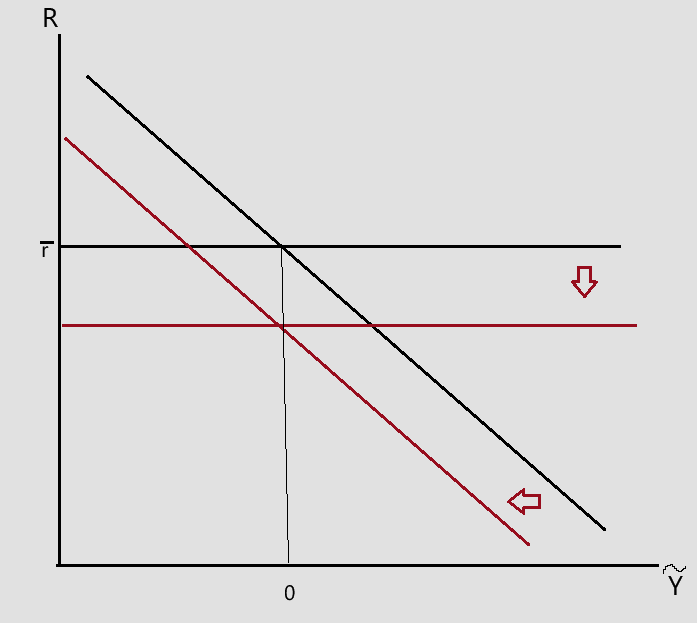
\includegraphics[width=0.45\linewidth]{figure/q31}
		\end{figure}
		
		
		\clearpage
		
		\textbf{(c) } 
		\begin{figure}[htbp!]
			\centering
			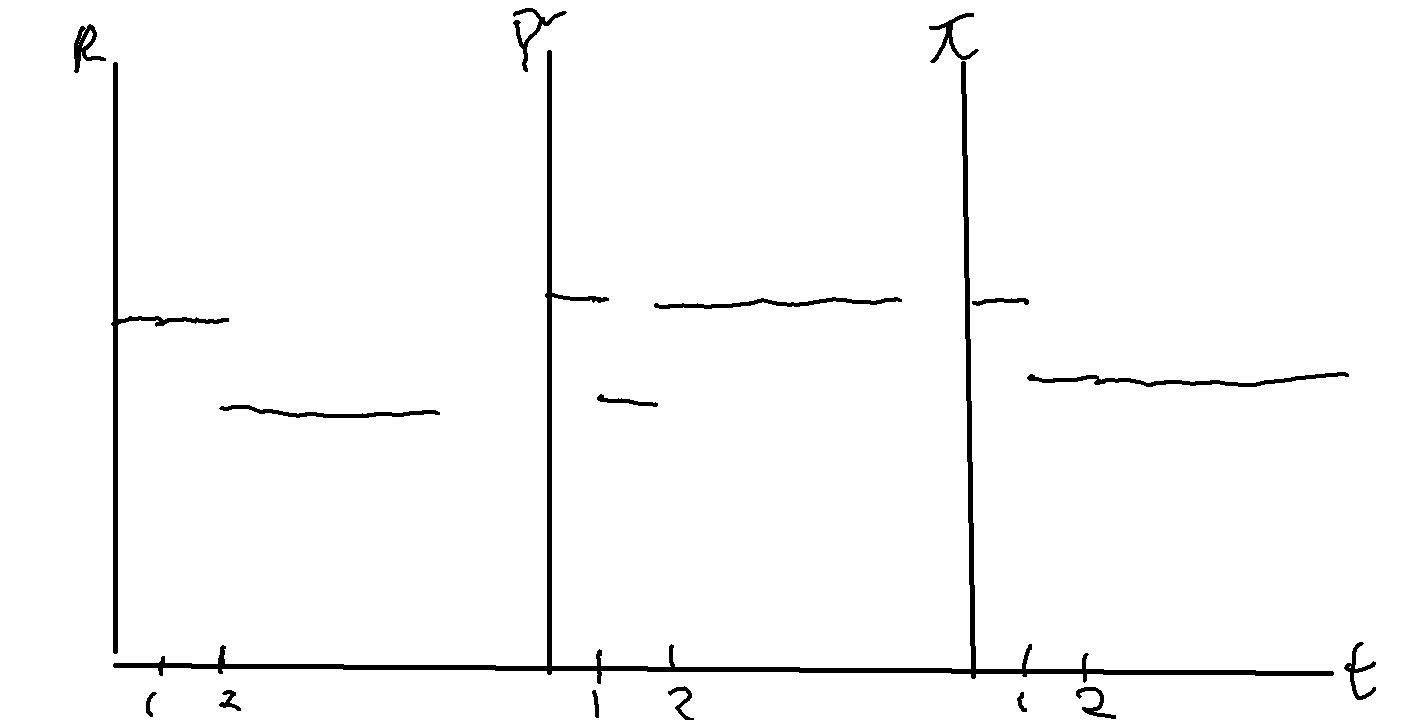
\includegraphics[width=0.7\linewidth]{figure/q3c}
		\end{figure}
		
		
		\medskip
		
		\textbf{(d) } 
		Substitute the Simple Monetary Rule into the IS equation to express the short run output in terms of inflation:
		\[
		\tilde{Y}_t = \frac{1}{1-\bar{x}}\left[\bar{a} - \bar{b}\left(\bar{m}(\pi_t-\bar{\pi})\right)\right].
		\]
		This equation represents the Aggregate Demand (AD) curve in the \((\pi,\tilde{Y})\) space. The Aggregate Supply (AS) curve is given by the Phillips curve:
		\[
		\pi_{t+1} = \pi_t + \bar{\nu}\tilde{Y}_t + \bar{o}.
		\]

		
		\medskip
		\clearpage
		\textbf{(e) } 
		A negative aggregate demand shock shifts the AD curve to the left, leading to a lower equilibrium output and a lower inflation rate in the short run. In the AD/AS diagram, there is a leftward shift from \(AD\) to \(AD'\). Then, given the negative $\tilde{Y}$, the inflation would move downward overtime. This would lead the economy moving from point B gradually to point C. In the longer run, the $\bar{a}$ has to be equal to zero. This means, the AD curve will move back to its initial position. This would lead the economy move from point C to point D. Then, gradually adjust to point A.
		
		\begin{figure}[htbp!]
			\centering
			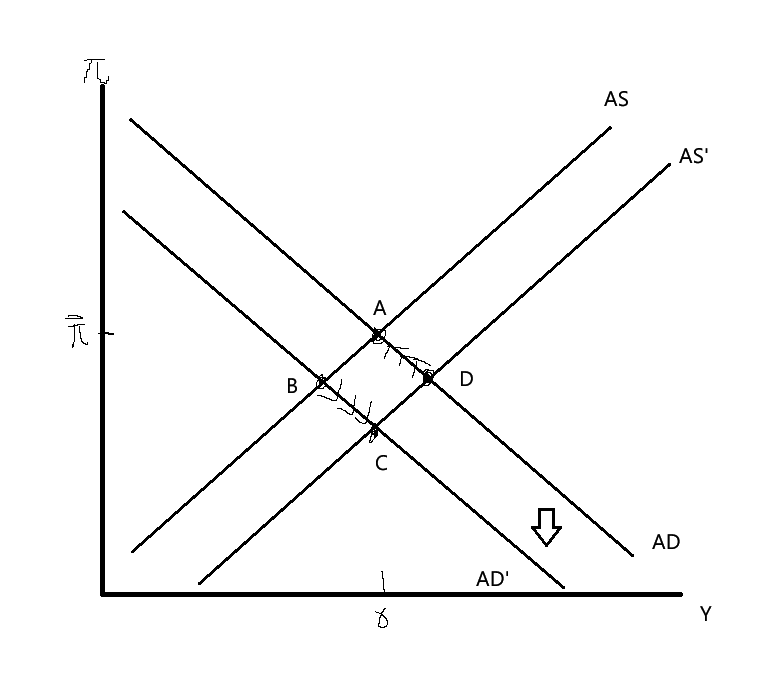
\includegraphics[width=0.7\linewidth]{figure/q3e}
		\end{figure}
		
				
		\medskip
		\clearpage
		\textbf{(f)} 
		
		\begin{figure}[htbp!]
			\centering
			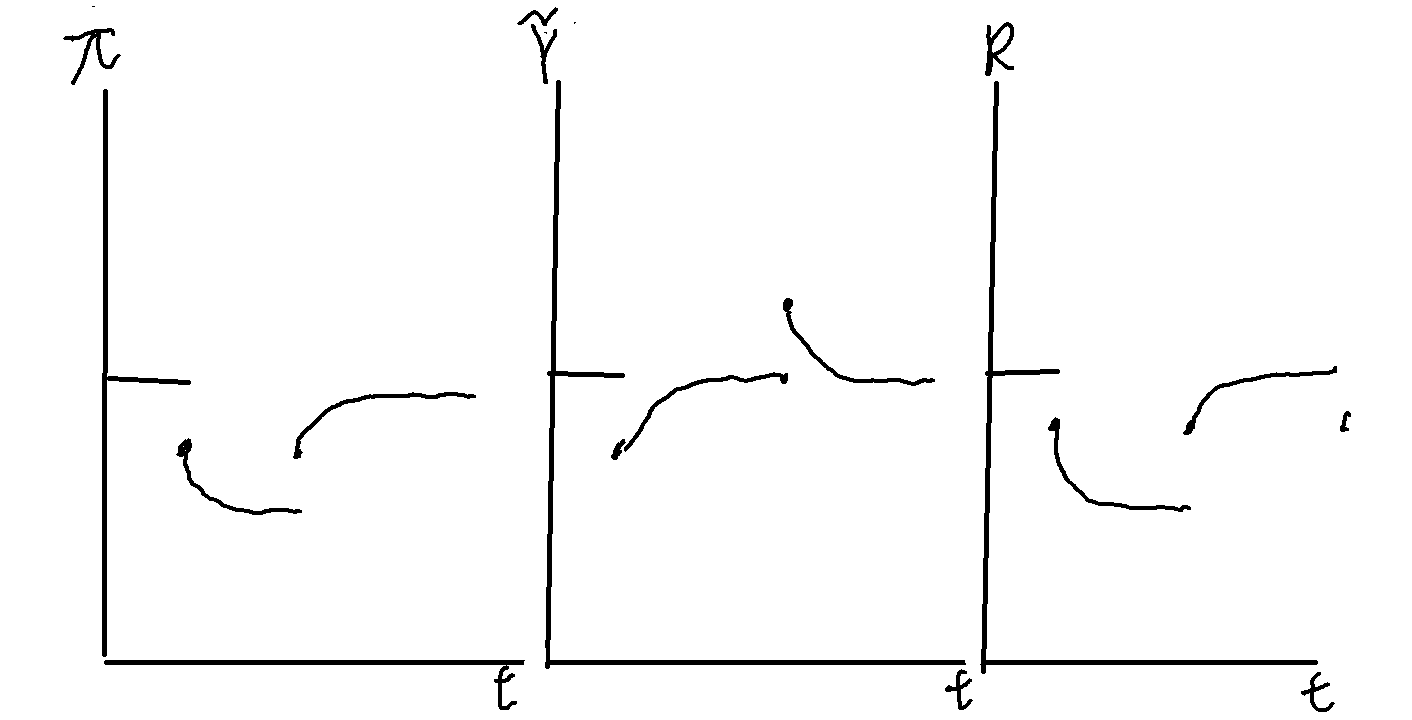
\includegraphics[width=0.7\linewidth]{figure/Q3f}
		\end{figure}
		
		\medskip
		
		\textbf{(g)} 		
		To reduce the inflation target from 3\% to 2\%, it can be represent by reducing the inflation target $\bar{\pi}$ from 3\% to 2\%. Based on the simple monetary rule, the central bank must increase the interest rate. This higher real interest rate reduces short run output, leading to a lower inflation rate over time. However, the cost of this tighter policy is a reduction in short-run output ()and possibly higher unemployment). In the AD/AS framework, the tightening of policy is represented by a leftward shift of the AD curve, which produces a new equilibrium with lower \(\pi\) but also lower \(\tilde{Y}\) in the short run. Then, it gradually move toward to the equilibrium with lower inflation and current production equal to the potential level.
		
		
		\begin{figure}[htbp!]
			\centering
			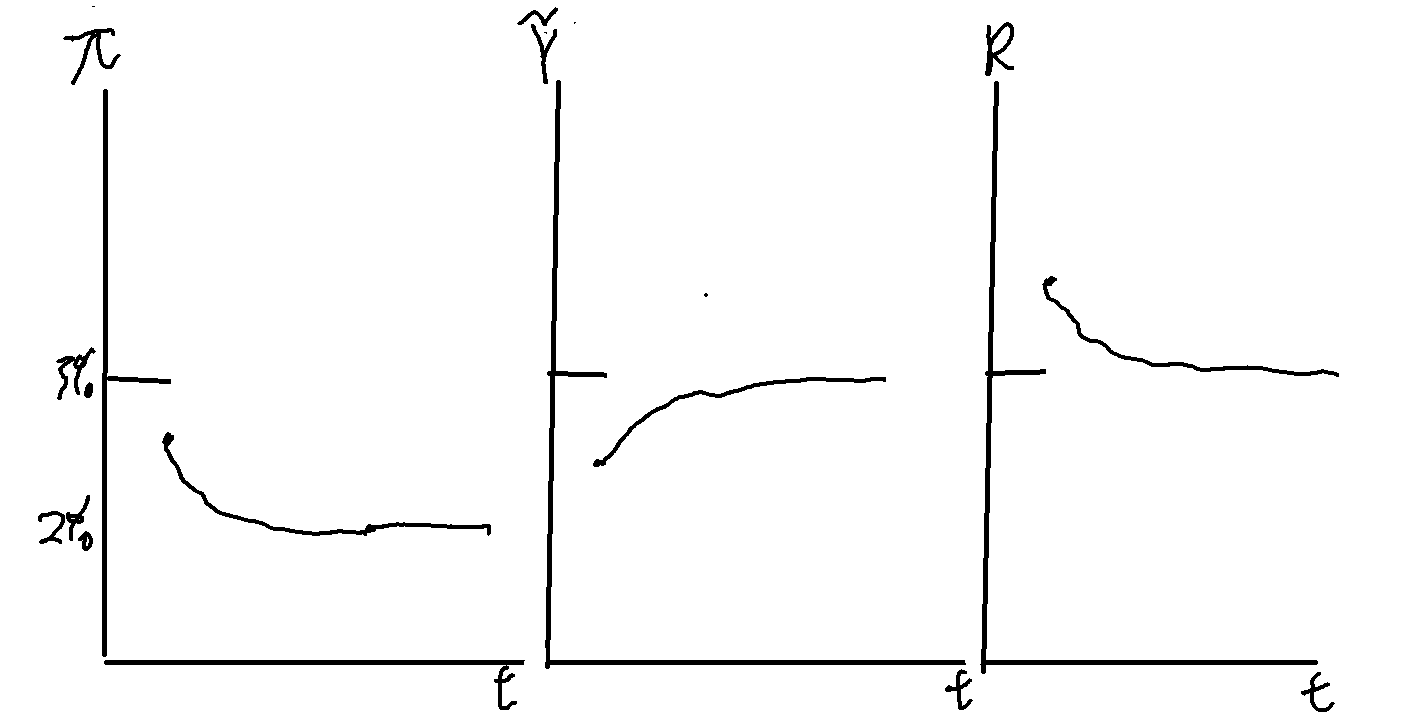
\includegraphics[width=0.7\linewidth]{figure/Q3g}
		\end{figure}
		
		%		

		

%		\newpage 
%		\centering{This page intentionally left blank.}
%		\ % The empty page
%		
		\vfill
		
		 \centering{-- The End -- }
		
		
		
		%		\begin{solution}
			%			
			%		\end{solution}	
%		\clearpage 
%		
%		\question Was wäre, wenn es keine Luft gäbe?
%		\begin{parts} 
%			\part[5] Was würde mit Luftballons geschehen? 
%			\bonuspart[6] Wie könnten Fluggesellschaften damit umgehen?
%		\end{parts}
%		
%		\question [100] Wird es morgen schneien?
%		\begin{checkboxes}
%			\CorrectChoice Ja
%			\choice Nein
%			\choice Vielleicht
%		\end{checkboxes}
%		
%		\question Ein Name der folgenden Reihe passt nicht zu den anderen. Welcher?
%		\begin{oneparchoices}
%			\choice Donald
%			\choice Dagobert
%			\choice Daisy
%			\choice Micky
%			\CorrectChoice Balu
%		\end{oneparchoices}
		
	\end{questions}
	
%	\begin{center}
%		\combinedgradetable[h][questions]
%	\end{center}
	
\end{document}